	La distribucion uniforme es una de las mas conocidas, y como la nomal, una de las mas presentes en la realidad.
	Esta distribucion es muy simple, basicamente plantea que si tenemos un espacio muestral $S=\{m_1, m_2, ... ,m_n\}$, $(\forall m_i \in S$,  $P(m_i)=1/n)$, osea, todos los sucesos tiene la misma probabilidad de ocurrir. 
			
	El ejemplo mas clasico para entender esa distribucion, es el lanzamiento de un dado de 6 caras (no cargado), en onde $S = \{1, 2, 3, 4, 5, 6\}$ y cada elemento tiene la misma probabilidad de salir, osea $1/6$.
			
\subsubsection*{Tiempo de espera de un colectivo}

	Otro ejemplo un poco mas interesante, es si tomamos un rango de tiempo, y medimos el tiempo de espera de un colectivo en ese rango de tiempo. Si bien este ejemplo dependera mucho de sobre que linea de colectivo hagamos el muestreo, se puede tomar un rango en particular en el cual sabemos que el tiempo de espera no sera mayor o menor a eso. A continuacion se presenta un histograma sobre un dataset sobre los tiempos de cierto colectivo en el rango de 5 minutos a 30 minutos.

\newpage					
	\begin{figure}[H]
	  \begin{center}
	    %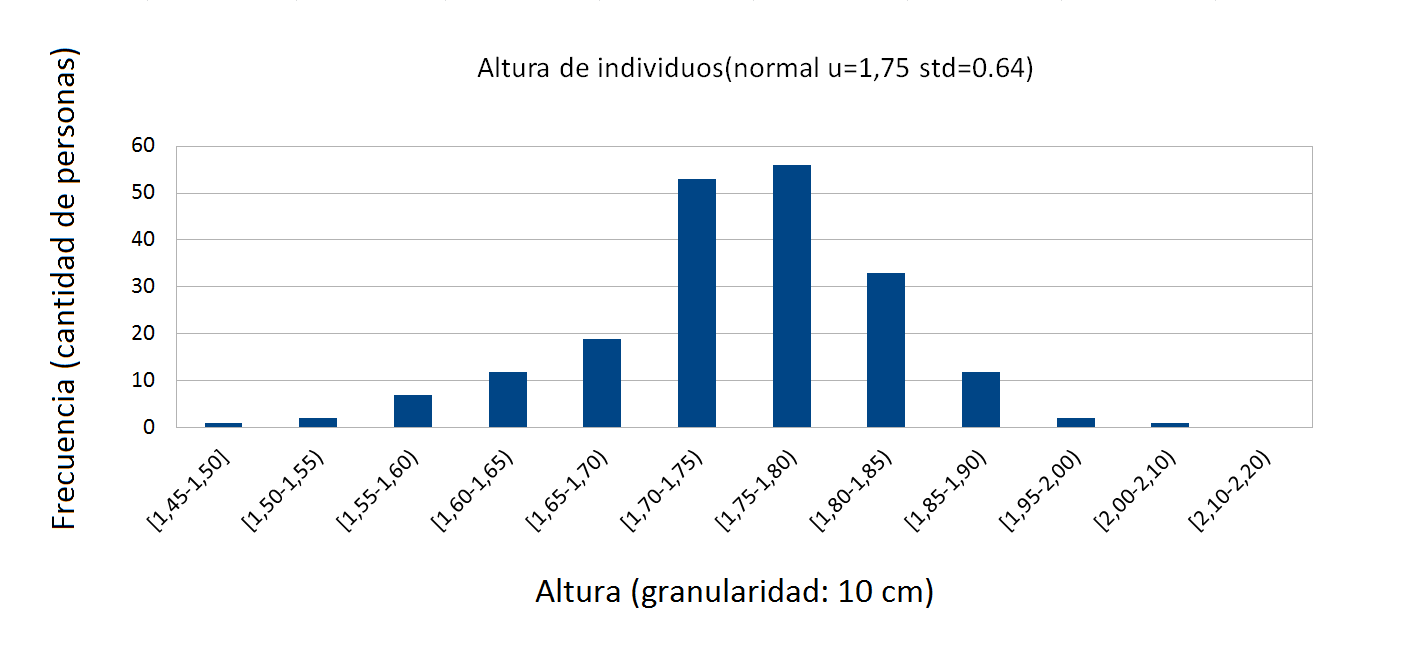
\includegraphics[scale=.41,angle=-90]{imgenes/normal_ejemplo1.png}
	    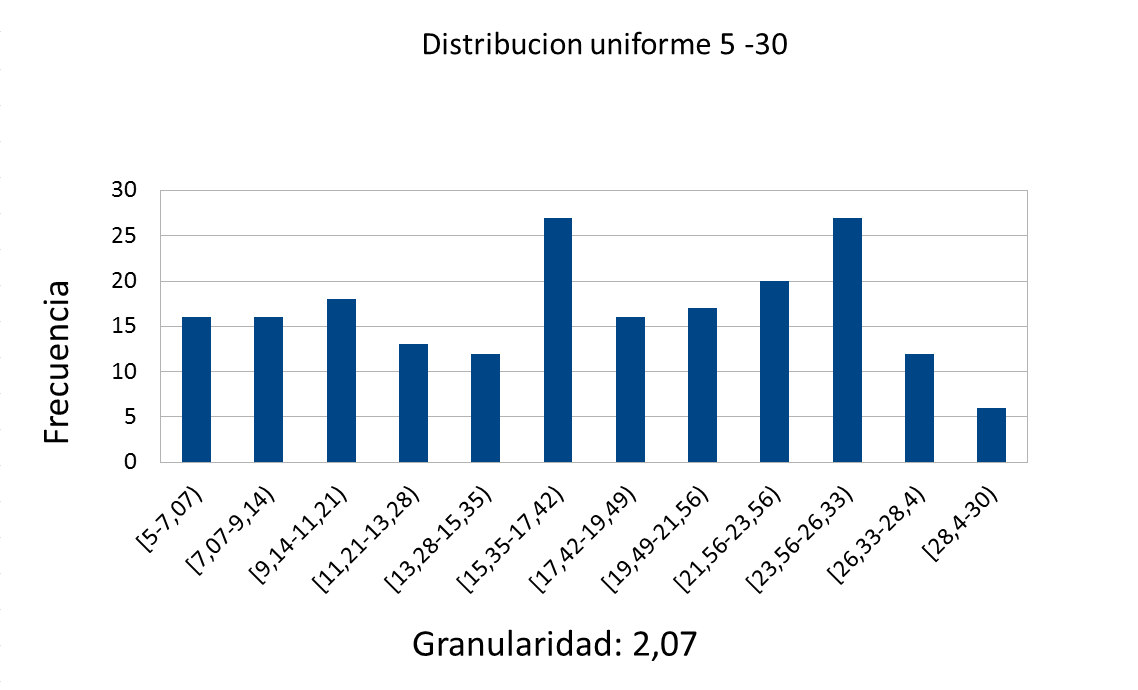
\includegraphics[scale=.40]{imagenes/uniforme_ejemplo.png}
	    \caption{Histograma tiempos de espera de colectivo} 
	    \label{fig:normal_ejemplo1}
	  \end{center}
	\end{figure}